\section{Описание использованного алгоритма}

\subsection{C использованием библиотечных функций}
\begin{figure}[H]
  \centering
  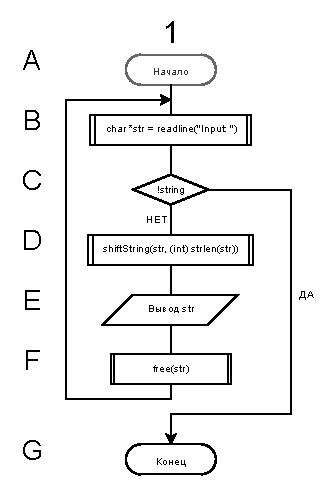
\includegraphics[width=0.25\textwidth]{fun_default}
  \caption{Блок-схема алгоритма работы функции \texttt{main()} в библиотеке \texttt{default}}
\end{figure}

\subsection{Без использования библиотечных функций}
\begin{figure}[H]
  \centering
  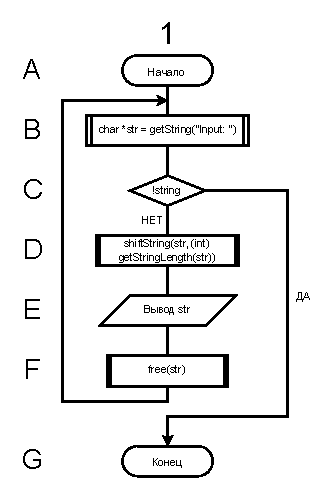
\includegraphics[width=0.25\textwidth]{fun_custom}
  \caption{Блок-схема алгоритма работы функции \texttt{main()} в библиотеке \texttt{custom}}
\end{figure}

\subsubsection{Аналоги функций из библиотеки \texttt{readline.h}}
\begin{figure}[H]
  \centering
  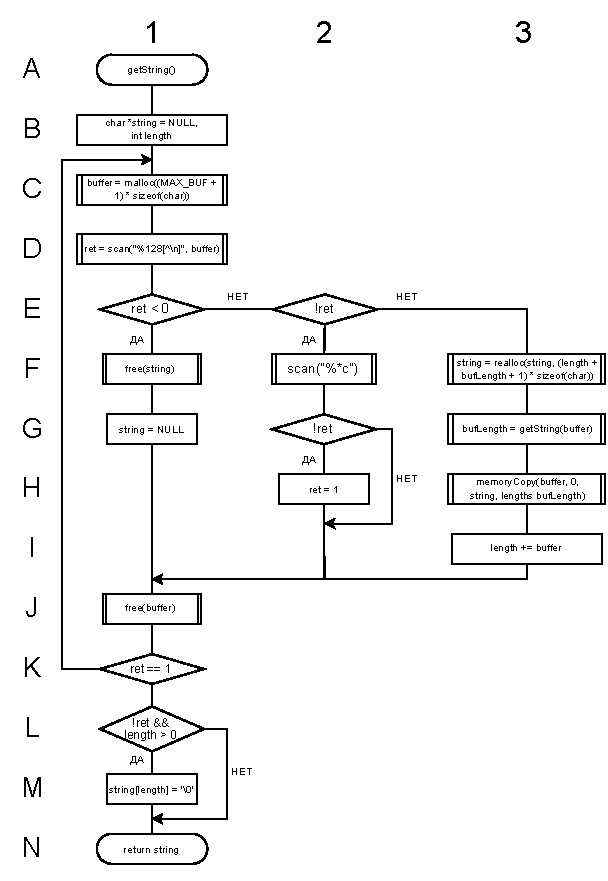
\includegraphics[width=0.55\textwidth]{fun_getString}
  \caption{Блок-схема алгоритма работы функции \texttt{getString()}}
\end{figure}

\subsubsection{Аналоги функций из библиотеки \texttt{string.h}}
\begin{figure}[H]
  \centering
  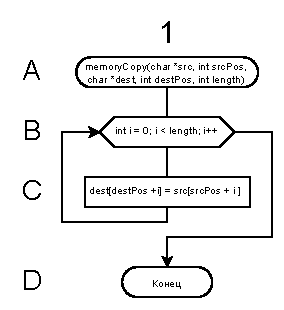
\includegraphics[width=0.3\textwidth]{fun_memoryCopy}
  \caption{Блок-схема алгоритма работы функции \texttt{memoryCopy()}}
\end{figure}
\begin{figure}[H]
  \centering
  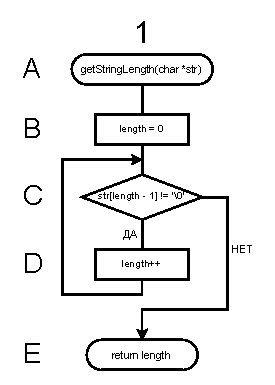
\includegraphics[width=0.275\textwidth]{fun_getStringLength}
  \caption{Блок-схема алгоритма работы функции \texttt{getStringLength()}}
\end{figure}

\subsection{Описание алгоритма модификации исходной строки}
\begin{figure}[H]
  \centering
  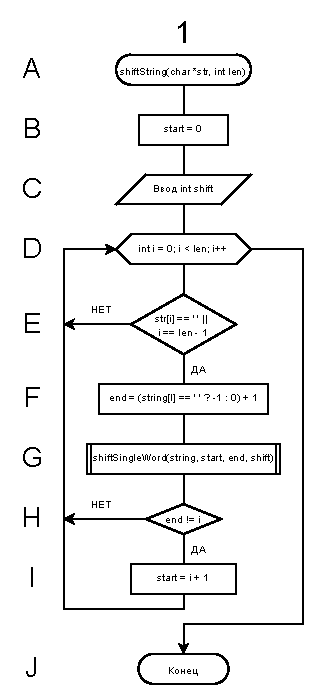
\includegraphics[width=0.35\textwidth]{fun_shiftString}
  \caption{Блок-схема алгоритма работы функции \texttt{shiftString()}}
\end{figure}
\begin{figure}[H]
  \centering
  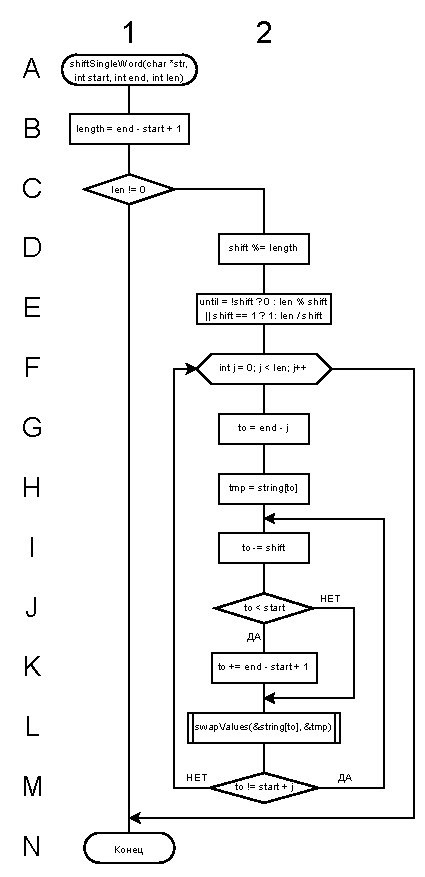
\includegraphics[width=0.55\textwidth]{fun_shiftSingleWord}
  \caption{Блок-схема алгоритма работы функции \texttt{shiftSingleWord()}}
\end{figure}
\begin{figure}[H]
  \centering
  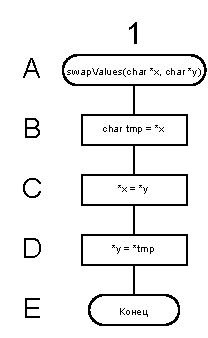
\includegraphics[width=0.25\textwidth]{fun_swapValues}
  \caption{Блок-схема алгоритма работы функции \texttt{swapValues()}}
\end{figure}
